\documentclass{article}

\usepackage{amsmath}
\usepackage{amssymb}
\usepackage{graphicx}

\graphicspath{ {./graphs/} }

\title{Week 01 and Week 02 Participation Assignment (2 of 4)}
\date{24 February 2023}
\author{Corey Mostero}

\begin{document}

\maketitle
\newpage

\tableofcontents

\section{Part 2}

\textbf{Directions:} Use a computer software to sketch the direction field for the following differential equations. Sketch some of the solution curves. (You may simply google "direction field graph". Then there should be several commonly used programs/websites such as geogebra, desmos). You can simply take a screen shot of the direction field.

\subsection{ $ \frac{dy}{dx} = \sin(x) $ }

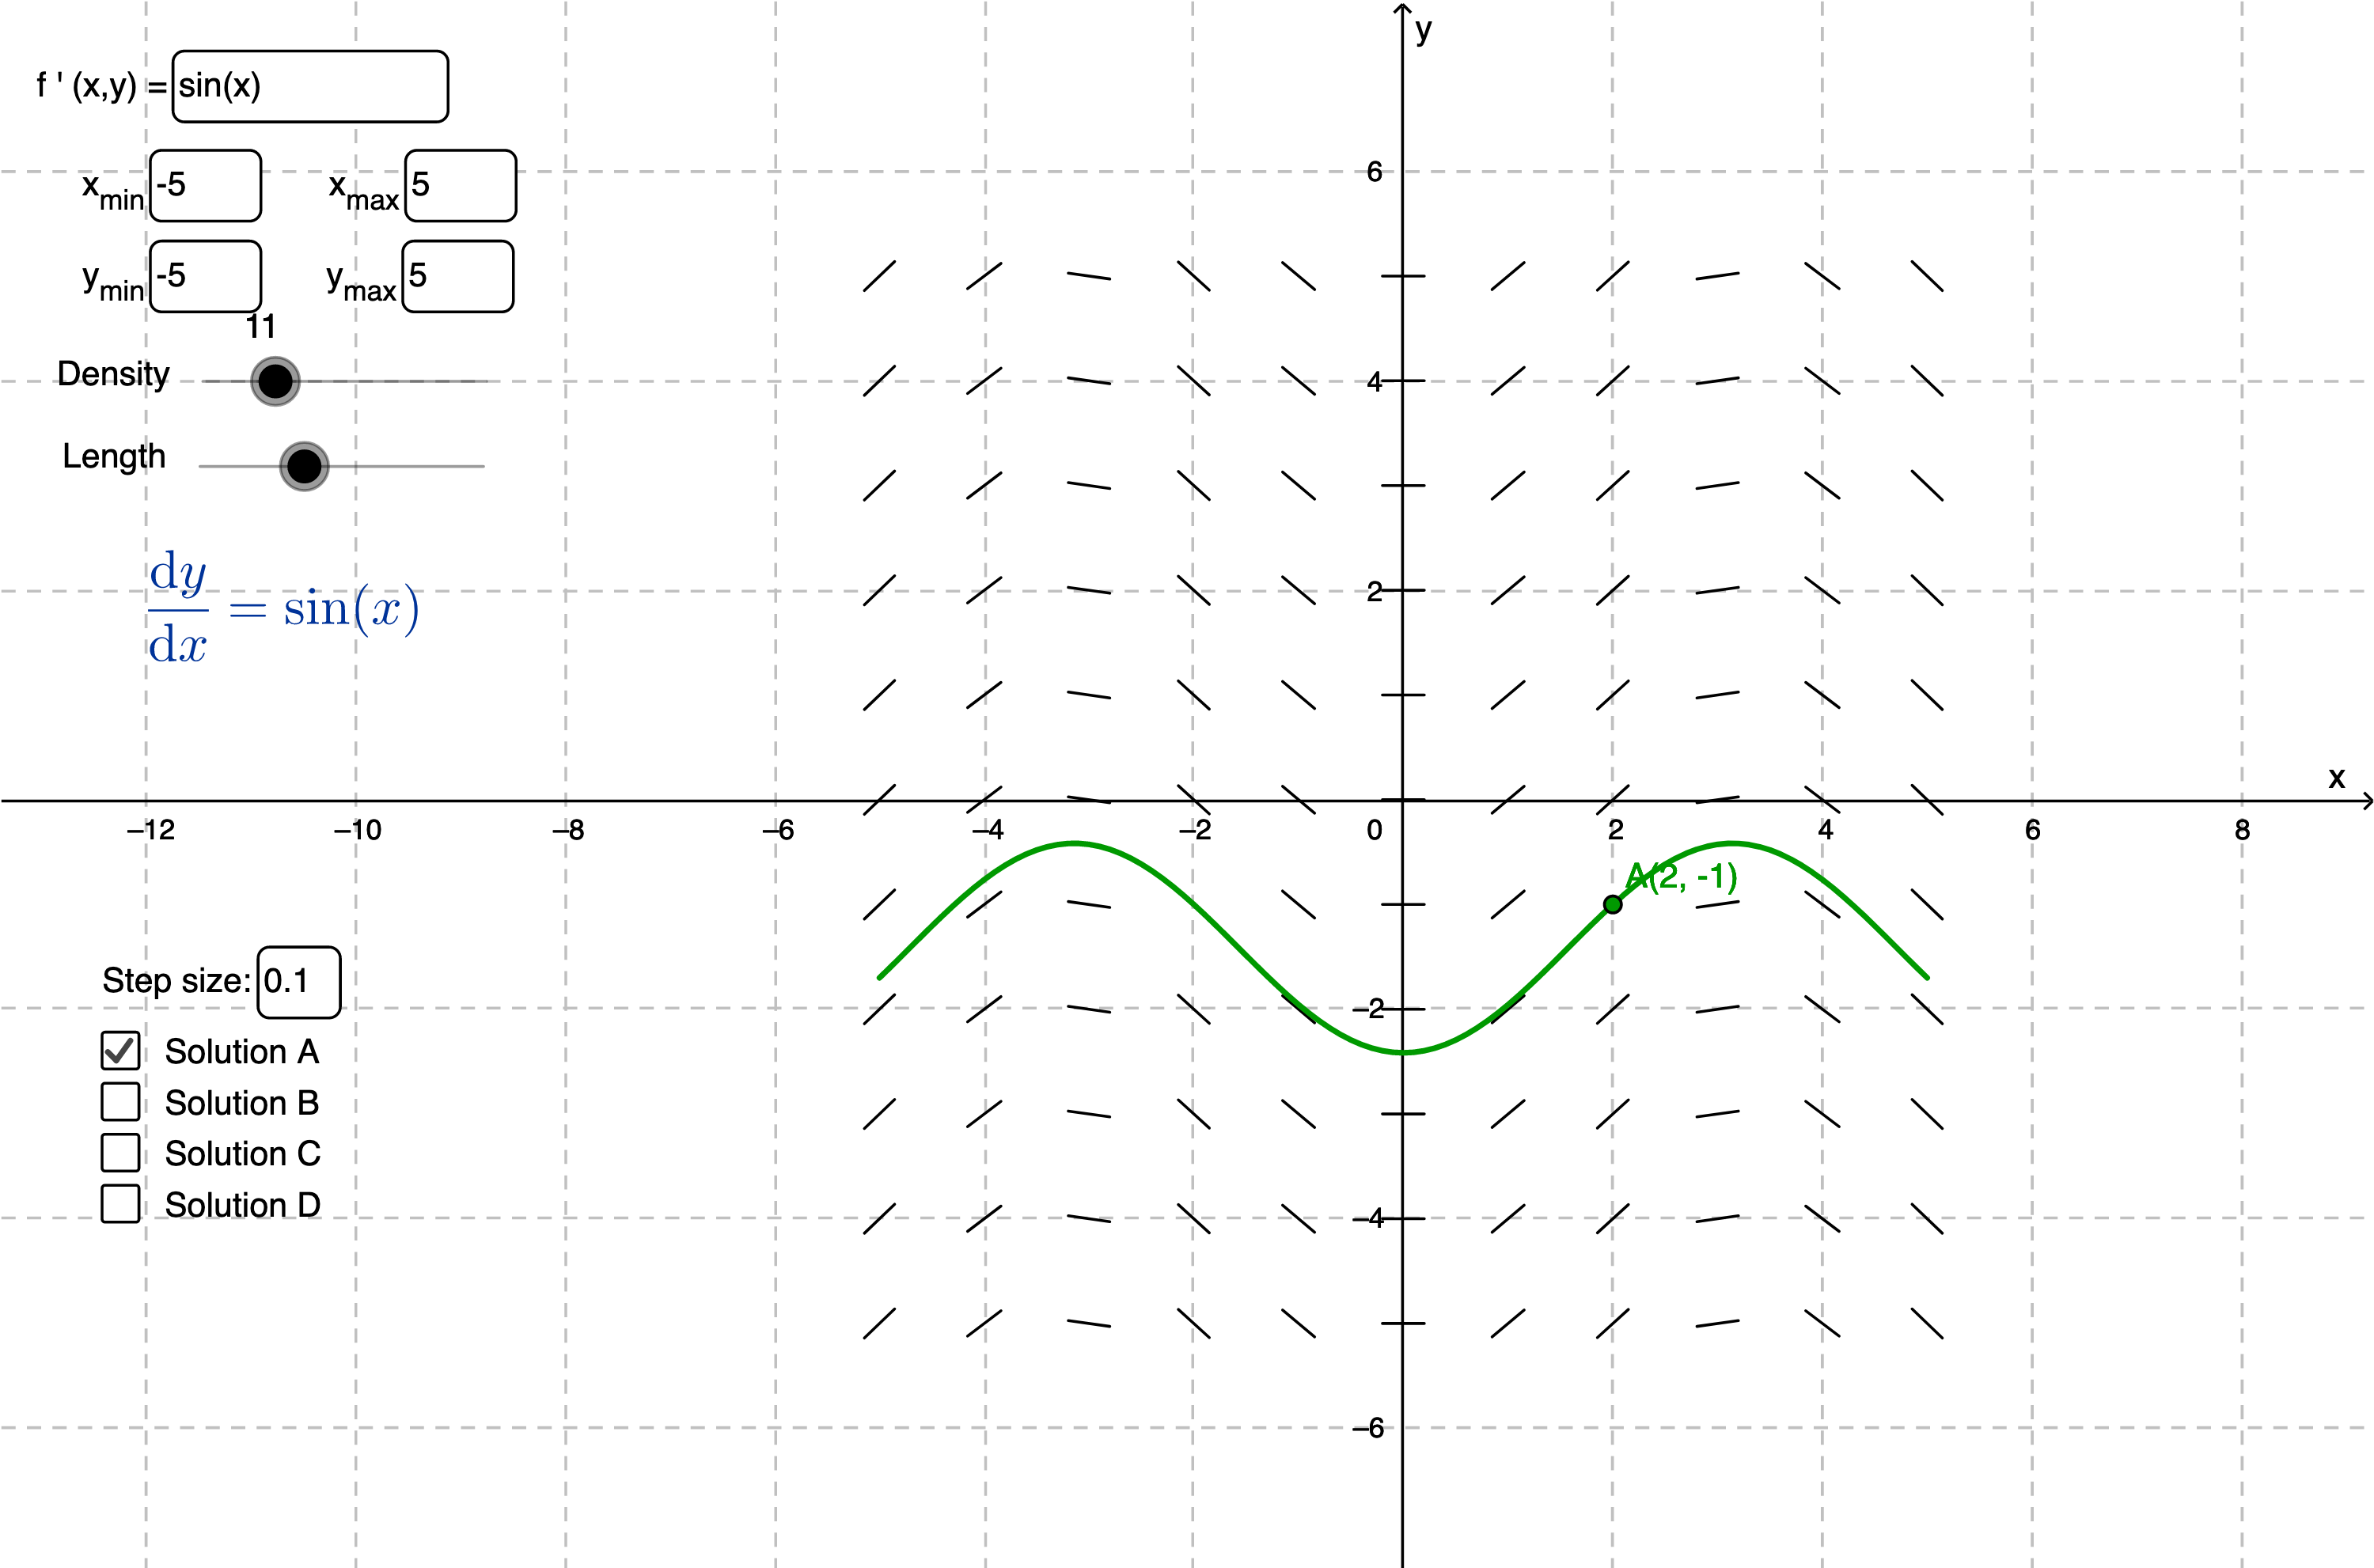
\includegraphics[width=\textwidth]{graph_1.png}

\subsection{ $ \frac{dy}{dx} = \sin(y) $ }

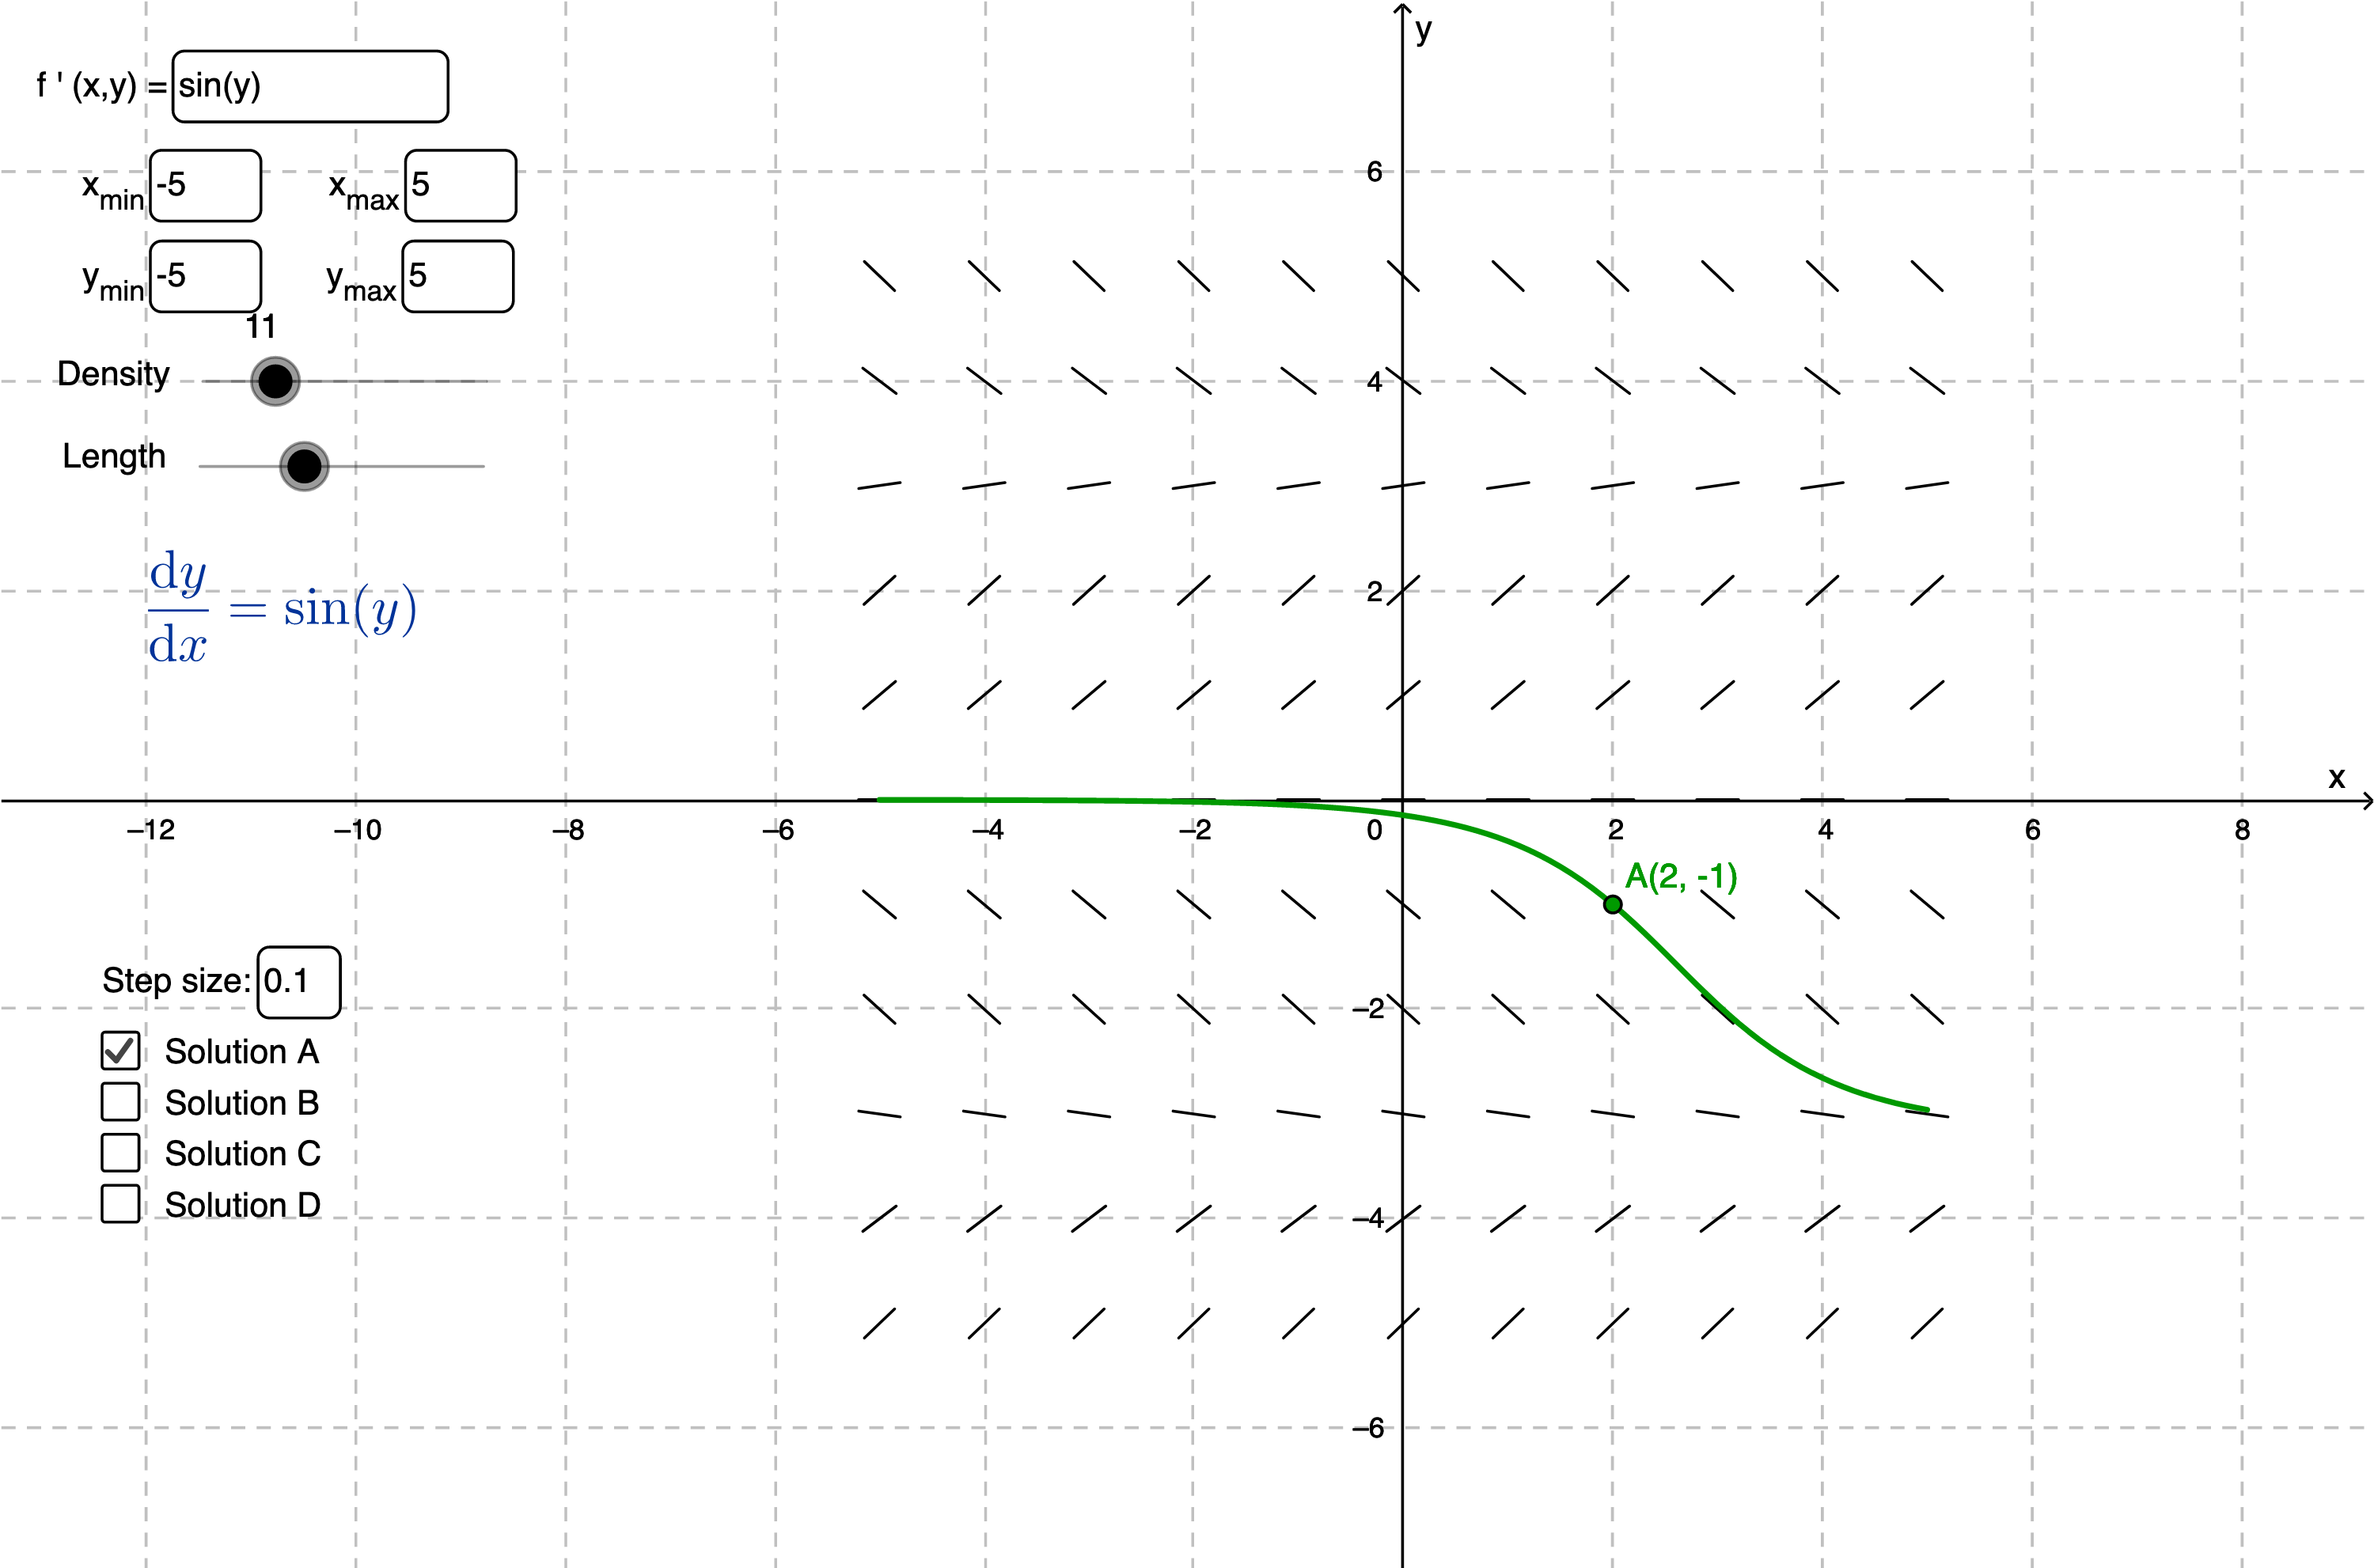
\includegraphics[width=\textwidth]{graph_2.png}

\subsection{ $ \frac{dy}{dx} = \sin(x)\sin(y) $ }

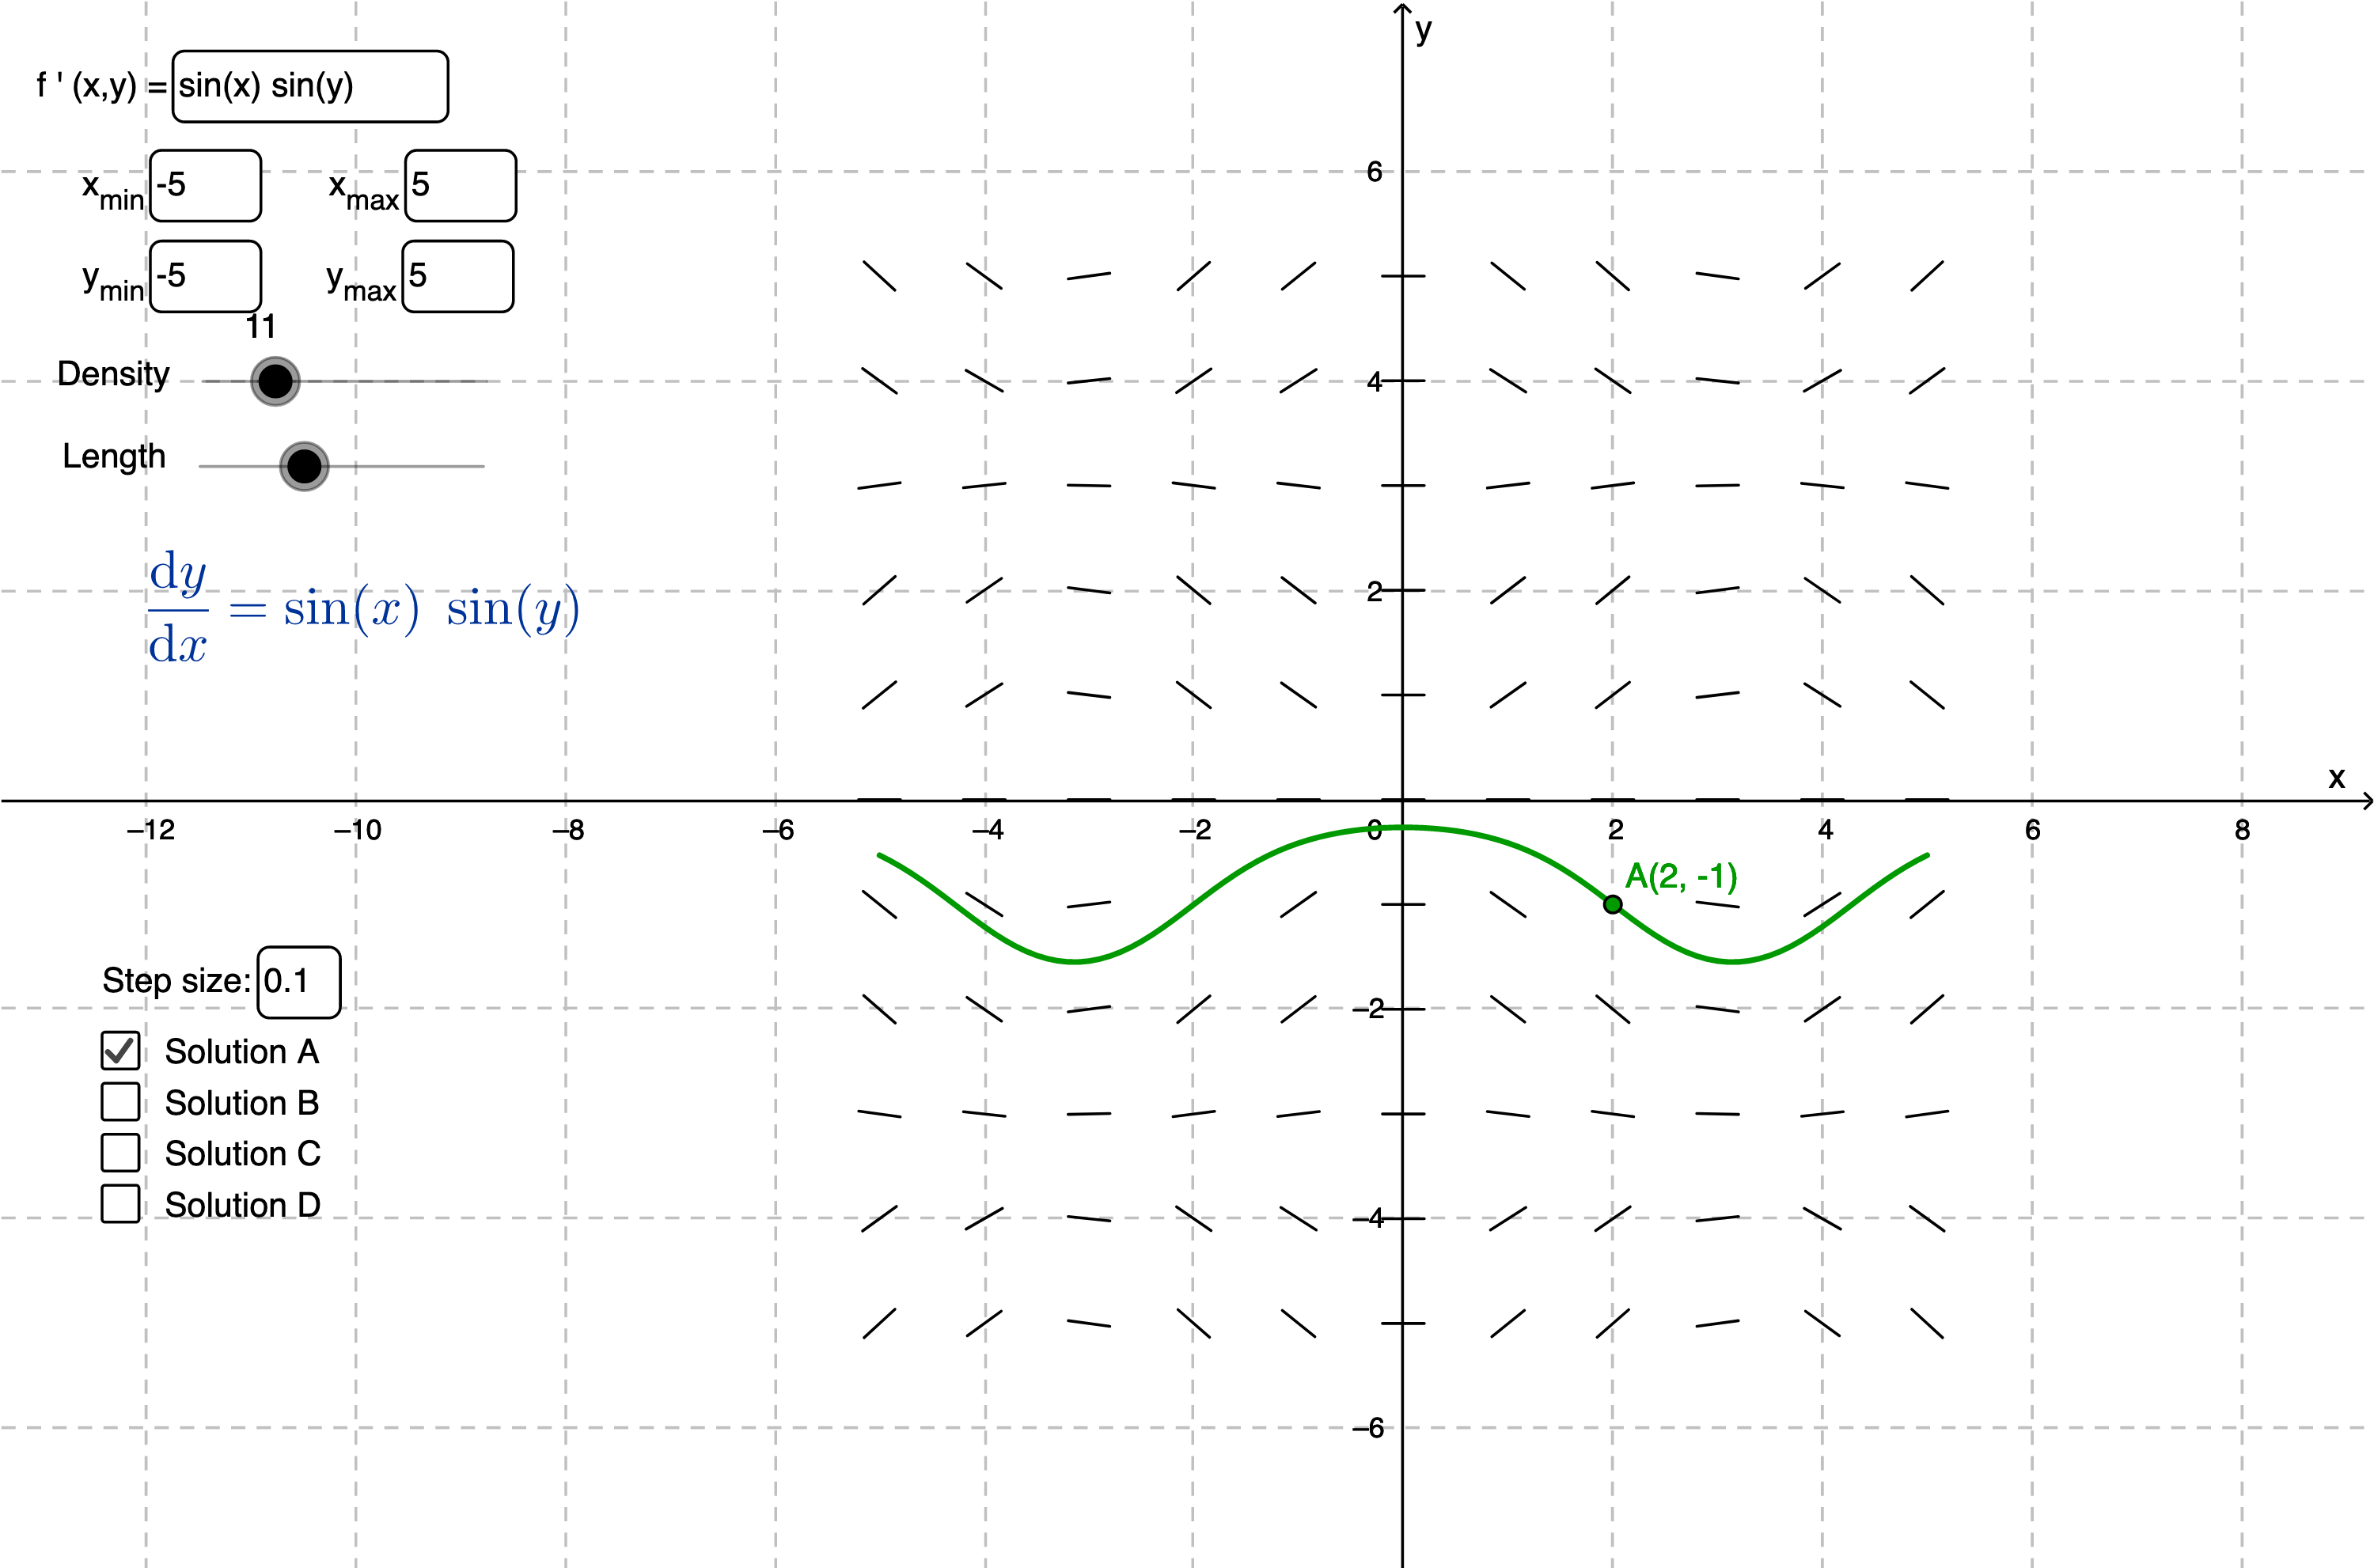
\includegraphics[width=\textwidth]{graph_3.png}

\subsection{ $ \frac{dy}{dx} = x^2 + 2y^2 $ }

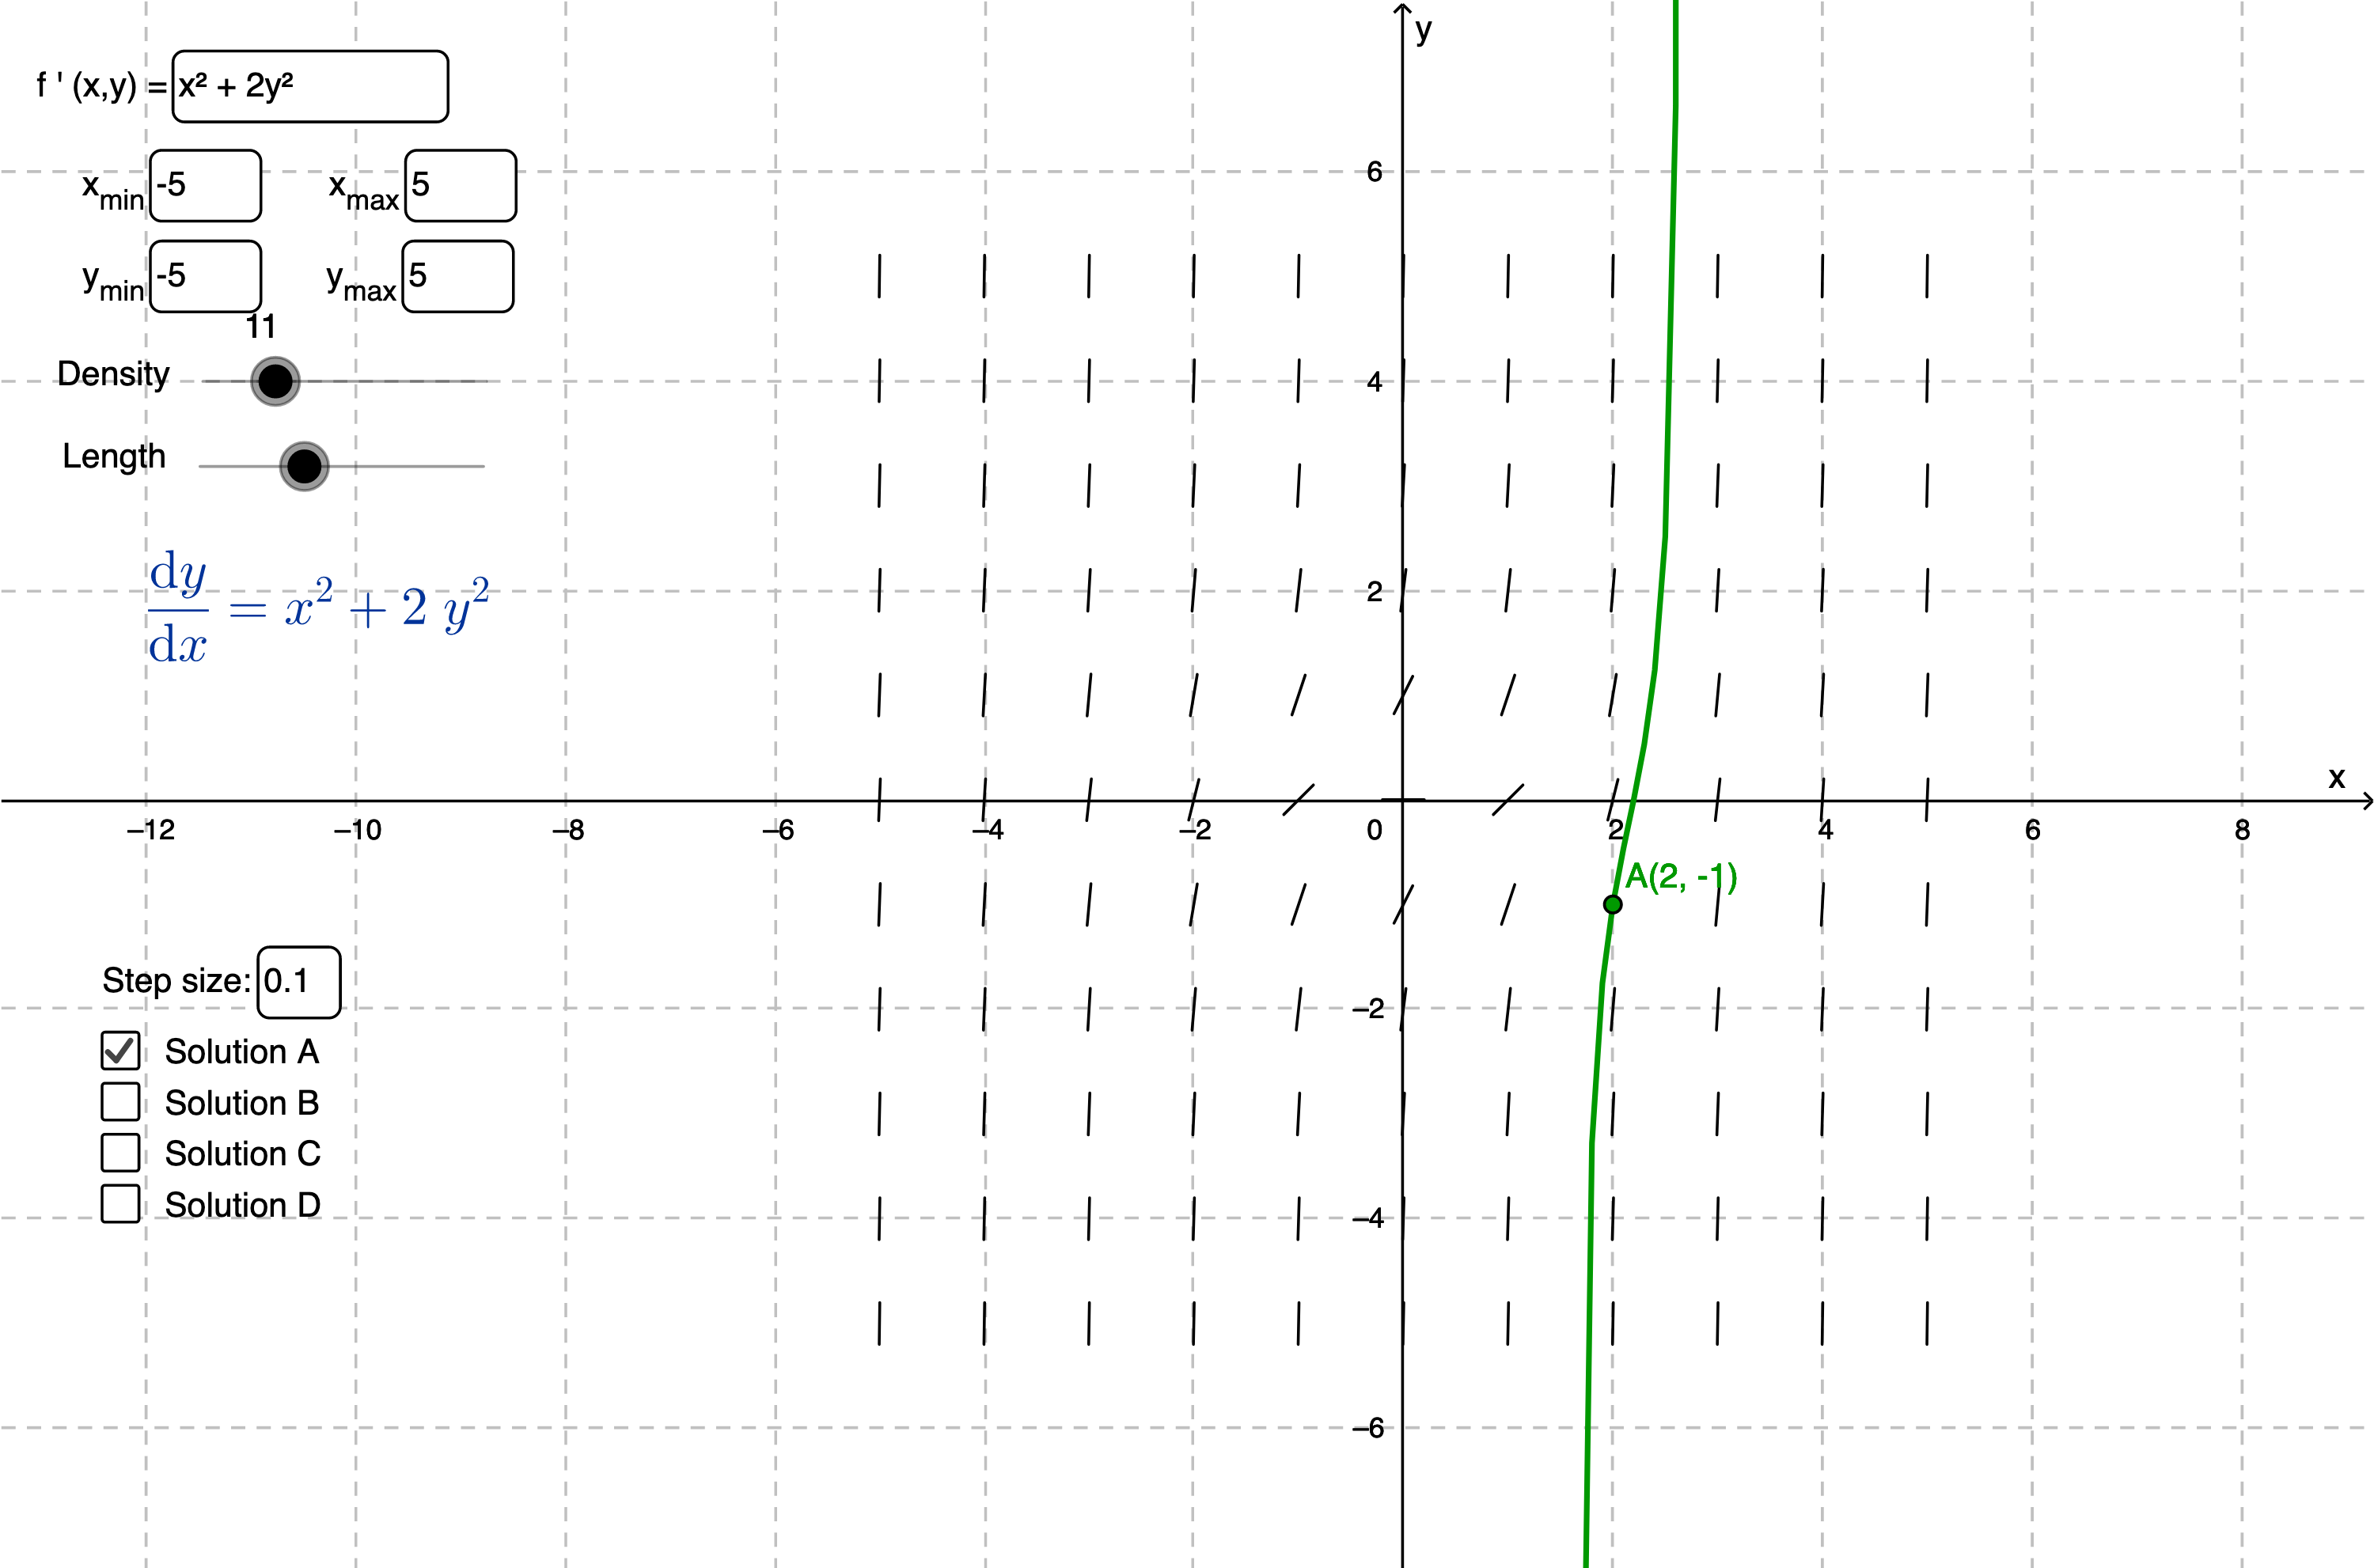
\includegraphics[width=\textwidth]{graph_4.png}

\subsection{ $ \frac{dy}{dx} = x^2 - 2y^2 $ }

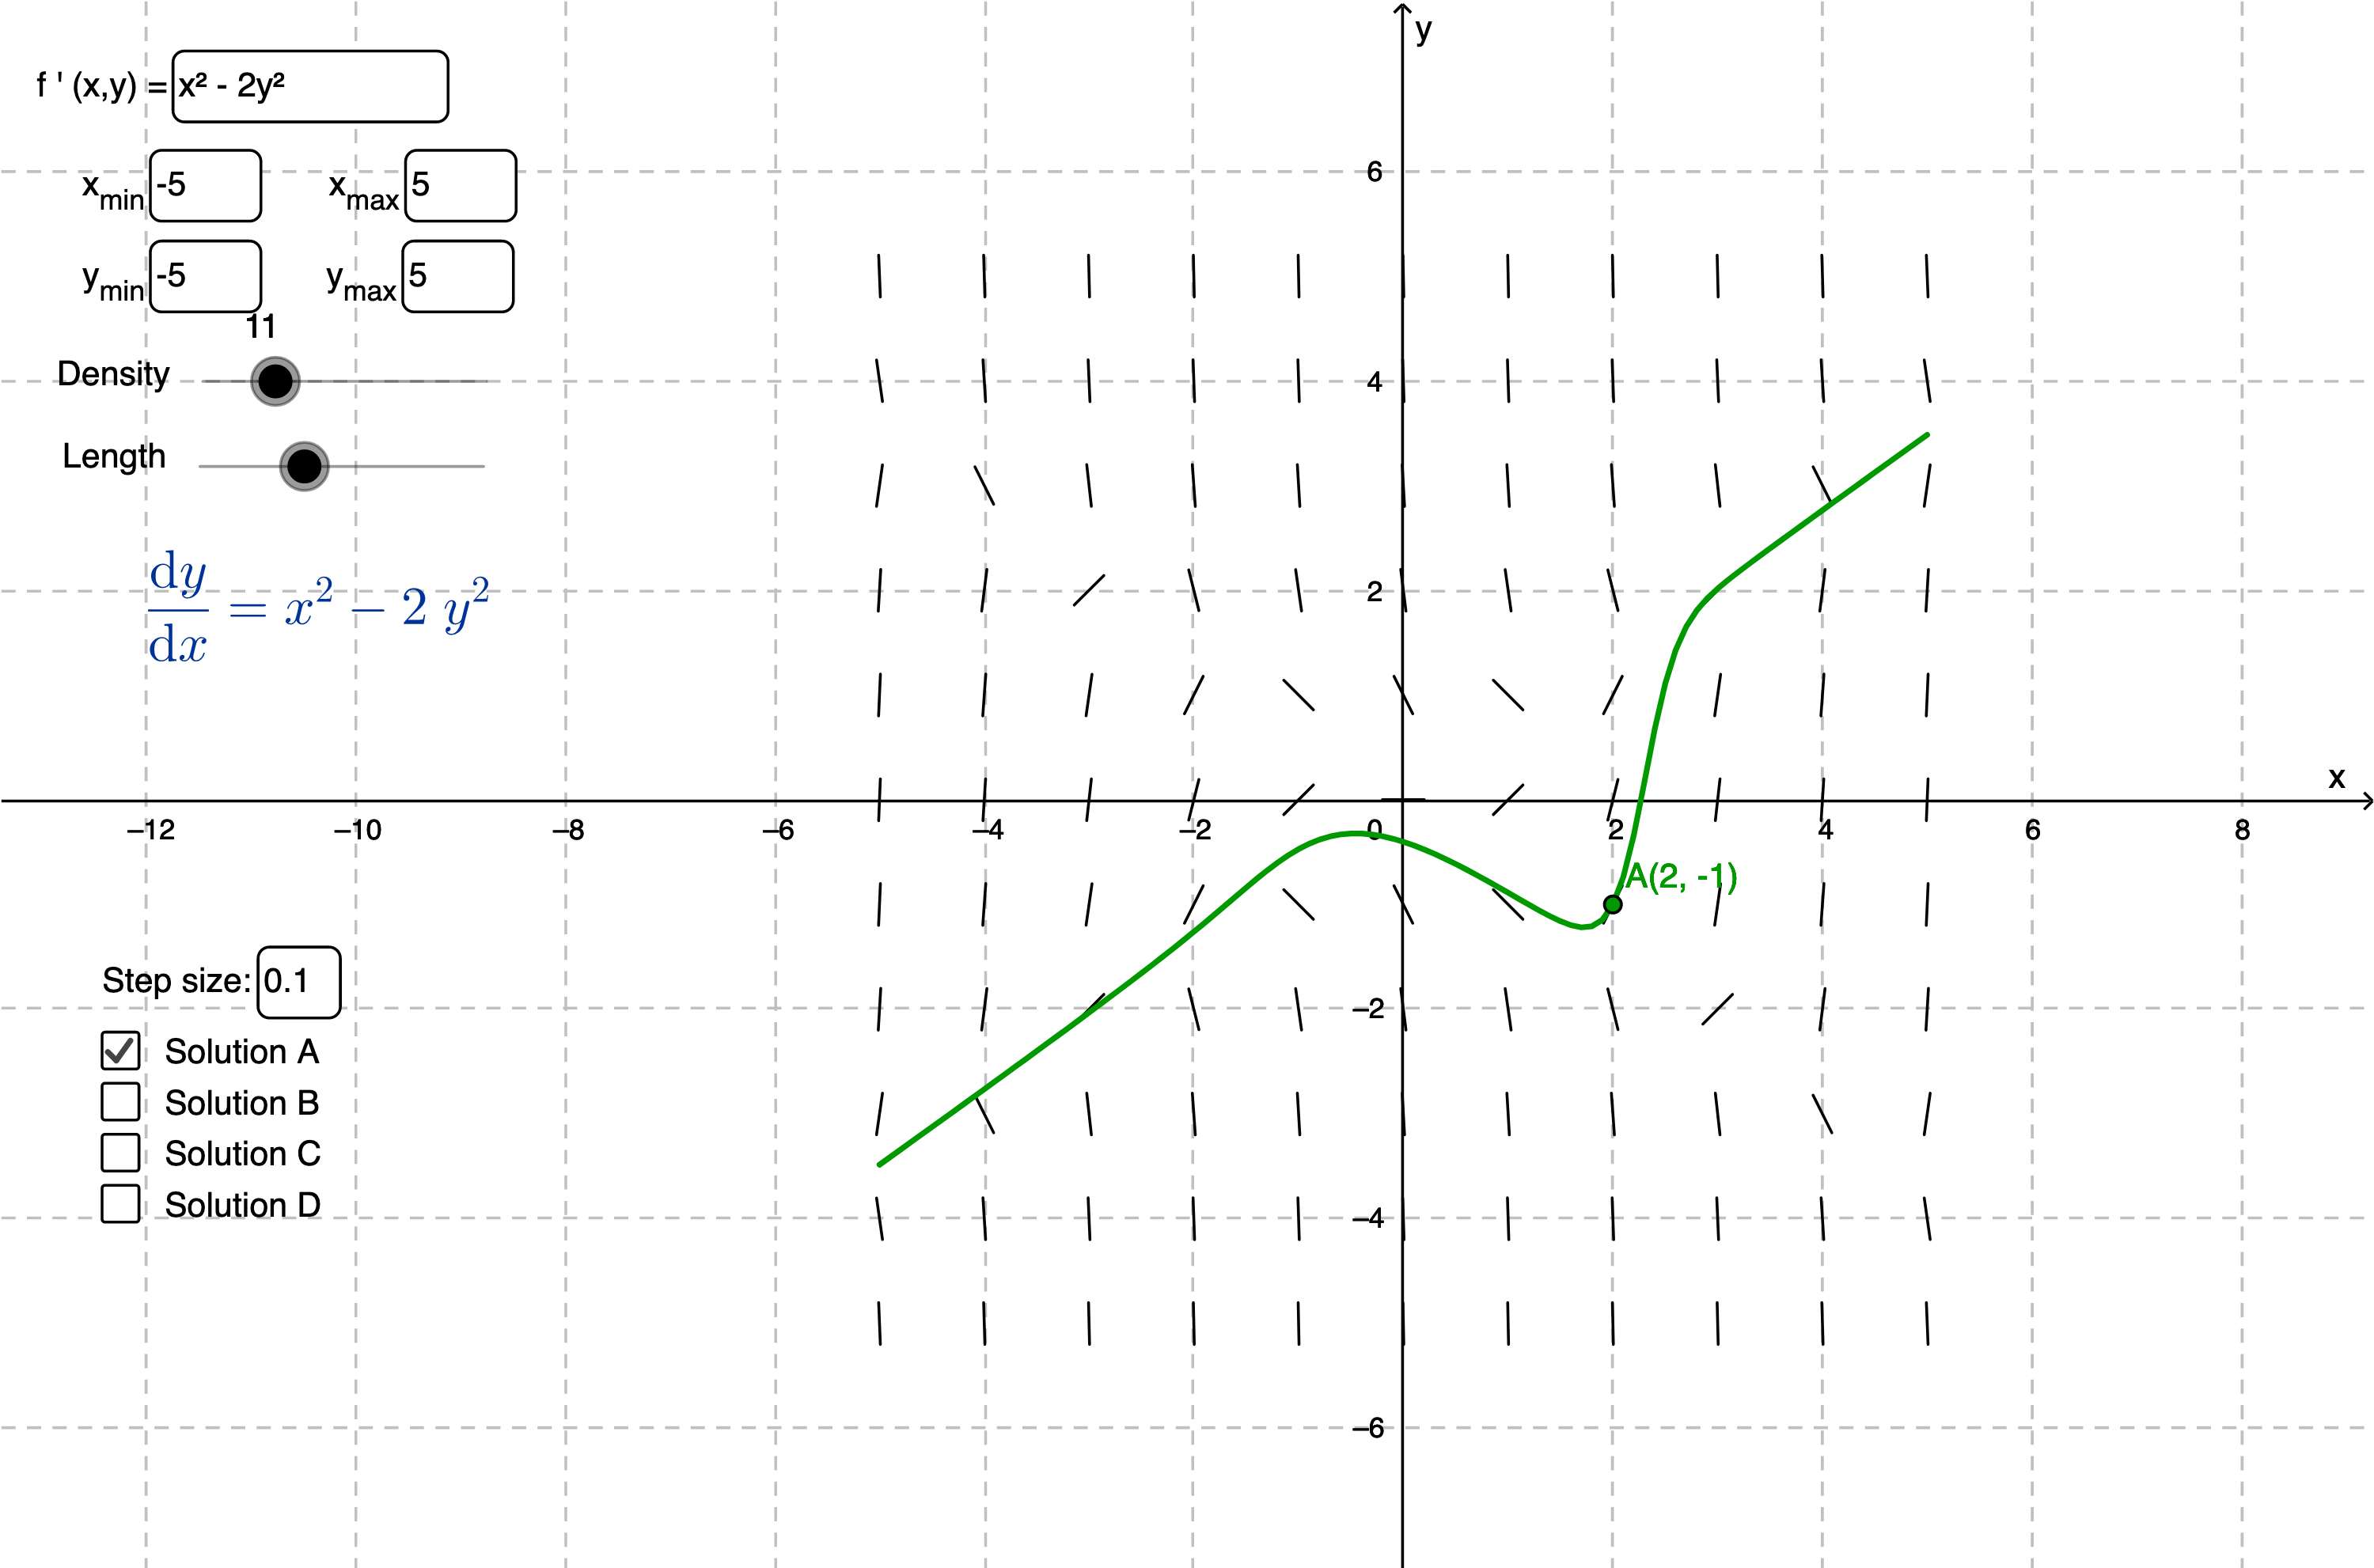
\includegraphics[width=\textwidth]{graph_5.png}

\end{document}
